% Generated from pipeline_layout.pptx; edit this TikZ source or the exporter label definitions.
% Uses the exact notation definitions and math font of the main manuscript.
\definecolor{pc0}{HTML}{FFEFE4}%
\definecolor{pc1}{HTML}{E58844}%
\definecolor{pc2}{HTML}{20252B}%
\definecolor{pc3}{HTML}{F5F1FB}%
\definecolor{pc4}{HTML}{7550AA}%
\definecolor{pc5}{HTML}{FFFFFF}%
\definecolor{pc6}{HTML}{D3D8DE}%
\definecolor{pc7}{HTML}{626B75}%
\definecolor{pc8}{HTML}{606872}%
\definecolor{pc9}{HTML}{CEBBE4}%
\definecolor{pc10}{HTML}{FFF7F1}%
\definecolor{pc11}{HTML}{F0BE96}%
\definecolor{pc12}{HTML}{626B78}%
\definecolor{pc13}{HTML}{DF5C12}%
\definecolor{pc14}{HTML}{FAFAFC}%
\definecolor{pc15}{HTML}{CFD4DE}%
\definecolor{pc16}{HTML}{ADB3BD}%
\definecolor{pc17}{HTML}{CABBDF}%
\definecolor{pc18}{HTML}{23272F}%
\definecolor{pc19}{HTML}{F4C4A4}%
\begin{tikzpicture}[x=1bp,y=-1bp]
\path[use as bounding box] (0,0) rectangle (1152.0000,635.0400);
\begin{scope}
% Aligned pseudo-labels / full-height generation panel
\path[fill=pc0,draw=pc1,line width=0.8500bp,rounded corners=8.770bp] (874.8000,59.0400) rectangle (1125.3600,362.8800);
% Panel a heading
\node[anchor=west,inner sep=0pt,text=pc2,font=\fontsize{26.00bp}{29.12bp}\selectfont] at (25.2000,28.0800) {\textbf{(a) Training}};
% Image–geometry alignment panel
\path[fill=pc3,draw=none,rounded corners=9.115bp] (308.8800,59.0400) rectangle (827.2800,362.8800);
% Alignment panel title
\node[anchor=west,inner sep=0pt,text=pc4,font=\fontsize{24.00bp}{26.88bp}\selectfont] at (329.0400,80.6400) {\textbf{Image--geometry alignment}};
% Unlabeled collection label
\node[anchor=center,inner sep=0pt,text=pc2,font=\fontsize{21.00bp}{23.52bp}\selectfont] at (87.4800,234.3600) {\textbf{Unlabeled}};
% Unlabeled real tactile image collection: rear card 2
\path[fill=pc5,draw=pc6,line width=0.6500bp] (36.0000,247.6800) rectangle (102.9600,314.6400);
% Unlabeled real tactile image collection: rear card 1
\path[fill=pc5,draw=pc6,line width=0.6500bp] (41.0400,252.0000) rectangle (108.0000,318.9600);
% Unlabeled real tactile image collection
\node[anchor=north west,inner sep=0pt] at (46.0800,256.3200) {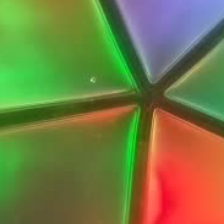
\includegraphics[width=66.9600bp,height=66.9600bp]{figures/pipeline_assets/asset_01.png}};
% Known input identity
\node[anchor=center,inner sep=0pt,text=pc7,font=\fontsize{20.00bp}{22.40bp}\selectfont] at (79.5600,337.3200) {$\Tactile,\,o$};
% Teacher module
\path[fill=pc5,draw=pc6,line width=0.8500bp,rounded corners=2.560bp] (151.2000,258.4800) rectangle (267.8400,315.3600);
% Unlabeled image to teacher
\draw[draw=pc8,line width=0.8500bp,line cap=round,-{Triangle[length=3.4bp,width=3bp]}] (118.0800,287.2800) -- (150.4799,287.2800);
% Teacher state to mesh projection
\draw[draw=pc8,line width=0.8500bp,line cap=round,-{Triangle[length=3.4bp,width=3bp]}] (268.5600,287.2800) -- (331.2000,287.2800);
% Initial state symbol
\node[anchor=center,inner sep=0pt,text=pc7,font=\fontsize{21.00bp}{23.52bp}\selectfont] at (298.8000,266.7600) {$q_0$};
% Object mesh
\node[anchor=north west,inner sep=0pt] at (337.6800,222.4800) {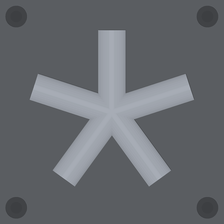
\includegraphics[width=27.3600bp,height=27.3600bp]{figures/pipeline_assets/asset_02.png}};
% Object mesh caption
\node[anchor=west,inner sep=0pt,text=pc7,font=\fontsize{19.00bp}{21.28bp}\selectfont] at (370.8000,235.4400) {Object mesh};
% Mesh input to projection
\draw[draw=pc8,line width=0.8000bp,line cap=round,-{Triangle[length=3.4bp,width=3bp]}] (351.3600,251.2799) -- (351.3600,257.7600);
% Real tactile image input to aligner
\node[anchor=north west,inner sep=0pt] at (596.1599,222.4800) {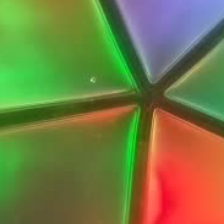
\includegraphics[width=27.3600bp,height=27.3600bp]{figures/pipeline_assets/asset_01.png}};
% Real tactile image caption
\node[anchor=west,inner sep=0pt,text=pc7,font=\fontsize{20.00bp}{22.40bp}\selectfont] at (631.4400,235.4400) {$\Tactile$};
% Real image input to aligner
\draw[draw=pc8,line width=0.8000bp,line cap=round,-{Triangle[length=3.4bp,width=3bp]}] (609.8400,251.2800) -- (609.8400,257.7600);
% Mesh projection module
\path[fill=pc5,draw=pc9,line width=0.8500bp,rounded corners=1.706bp] (331.9200,258.4800) rectangle (457.2000,315.3600);
% Projection label
\node[anchor=center,inner sep=0pt,text=pc2,font=\fontsize{21.00bp}{23.52bp}\selectfont] at (394.5600,275.0400) {\textbf{Projection}};
% Projection map
\node[anchor=center,inner sep=0pt,text=pc7,font=\fontsize{20.00bp}{22.40bp}\selectfont] at (394.5600,301.3200) {$d(\Mesh,q_t)$};
% Residual aligner module
\path[fill=pc5,draw=pc4,line width=1.2000bp,rounded corners=1.706bp] (505.4400,258.4800) rectangle (636.4800,315.3600);
% Residual aligner label
\node[anchor=center,inner sep=0pt,text=pc4,font=\fontsize{22.00bp}{24.64bp}\selectfont] at (570.9600,286.2000) {\textbf{Aligner}~$\Aligner$};
% State update module
\path[fill=pc5,draw=pc9,line width=0.8500bp,rounded corners=1.706bp] (692.6400,258.4800) rectangle (806.4000,315.3600);
% State update label
\node[anchor=center,inner sep=0pt,text=pc2,font=\fontsize{21.00bp}{23.52bp}\selectfont] at (749.5200,275.0400) {\textbf{Update}};
% Generic state update
\node[anchor=center,inner sep=0pt,text=pc7,font=\fontsize{17.50bp}{19.60bp}\selectfont] at (749.5200,300.9600) {$q_{t+1}=q_t+\Delta q$};
% Candidate projected depth to aligner
\draw[draw=pc8,line width=0.8500bp,line cap=round,-{Triangle[length=3.4bp,width=3bp]}] (457.2000,287.2800) -- (504.7200,287.2800);
% Residual correction to update
\draw[draw=pc8,line width=0.8500bp,line cap=round,-{Triangle[length=3.4bp,width=3bp]}] (637.2000,287.2800) -- (691.9200,287.2800);
% Residual symbol
\node[anchor=center,inner sep=0pt,text=pc7,font=\fontsize{20.00bp}{22.40bp}\selectfont] at (663.8400,267.8400) {$\Delta q$};
% Iterative alignment feedback / 1
\draw[draw=pc4,line width=0.8000bp,line cap=round] (749.5200,316.8000) -- (749.5200,341.2800);
% Iterative alignment feedback / 2
\draw[draw=pc4,line width=0.8000bp,line cap=round] (749.5200,341.2800) -- (394.5600,341.2800);
% Iterative alignment feedback / 3
\draw[draw=pc4,line width=0.8000bp,line cap=round,-{Triangle[length=3.4bp,width=3bp]}] (394.5600,341.2800) -- (394.5600,316.8000);
% Feedback label backing
\path[fill=pc3,draw=none] (477.3600,329.0400) rectangle (668.1600,352.0800);
% Generic iteration label
\node[anchor=center,inner sep=0pt,text=pc4,font=\fontsize{19.00bp}{21.28bp}\selectfont] at (572.7600,339.4800) {Iterative refinement};
% All real tactile images collection: rear card 2
\path[fill=pc5,draw=pc6,line width=0.6500bp] (47.5200,386.6400) rectangle (92.1600,431.2800);
% All real tactile images collection: rear card 1
\path[fill=pc5,draw=pc6,line width=0.6500bp] (52.5600,390.9600) rectangle (97.2000,435.6000);
% All real tactile images collection
\node[anchor=north west,inner sep=0pt] at (57.6000,395.2800) {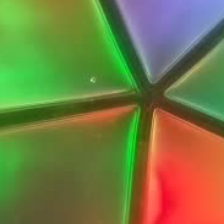
\includegraphics[width=44.6400bp,height=44.6400bp]{figures/pipeline_assets/asset_01.png}};
% All real images collection caption
\node[anchor=center,inner sep=0pt,text=pc2,font=\fontsize{20.00bp}{22.40bp}\selectfont] at (88.2000,458.6400) {All real images};
% Real training images to student
\draw[draw=pc8,line width=0.8500bp,line cap=round,-{Triangle[length=3.4bp,width=3bp]}] (108.0000,419.0400) -- (194.4000,419.0400);
% Student training module
\path[fill=pc5,draw=pc6,line width=0.8500bp,rounded corners=1.814bp] (195.8400,389.5200) rectangle (357.8400,450.0000);
% Geometric training targets panel
\path[fill=pc0,draw=pc1,line width=1.0000bp,rounded corners=2.354bp] (599.7600,386.6400) rectangle (1125.3600,465.1200);
% Registered label depth example
\node[anchor=north west,inner sep=0pt] at (646.5600,396.7200) {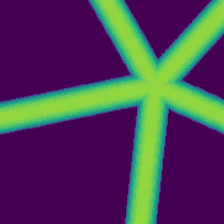
\includegraphics[width=36.0000bp,height=36.0000bp]{figures/pipeline_assets/asset_03.png}};
% Registered label normal example
\node[anchor=north west,inner sep=0pt] at (691.9200,396.7200) {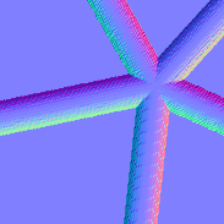
\includegraphics[width=36.0000bp,height=36.0000bp]{figures/pipeline_assets/asset_04.png}};
% Registered planar-pose target schematic / background
\path[fill=pc10,draw=pc11,line width=0.8000bp,rounded corners=0.900bp] (737.2800,396.7200) rectangle (773.2800,432.7200);
% Registered planar-pose target schematic / x axis
\draw[draw=pc12,line width=1.0000bp,line cap=round,-{Triangle[length=3.4bp,width=3bp]}] (745.9200,424.4400) -- (767.1600,424.4400);
% Registered planar-pose target schematic / y axis
\draw[draw=pc12,line width=1.0000bp,line cap=round,-{Triangle[length=3.4bp,width=3bp]}] (745.9200,424.4400) -- (745.9200,402.4800);
% Registered planar-pose target schematic / pose frame 0
\draw[draw=pc13,line width=1.0000bp,line cap=round] (748.4174,414.4587) -- (762.6121,405.9297);
% Registered planar-pose target schematic / pose frame 1
\draw[draw=pc13,line width=1.0000bp,line cap=round] (762.6121,405.9297) -- (765.0225,409.9412);
% Registered planar-pose target schematic / pose frame 2
\draw[draw=pc13,line width=1.0000bp,line cap=round] (765.0225,409.9412) -- (750.8278,418.4702);
% Registered planar-pose target schematic / pose frame 3
\draw[draw=pc13,line width=1.0000bp,line cap=round] (750.8278,418.4702) -- (748.4174,414.4587);
% Registered planar-pose target schematic / origin
\path[fill=pc13,draw=pc13,line width=1.0000bp] (745.9199,424.4399) ellipse [x radius=0.9720bp,y radius=0.9720bp];
% Registered targets caption
\node[anchor=center,inner sep=0pt,text=pc13,font=\fontsize{20.00bp}{22.40bp}\selectfont] at (709.9200,451.4400) {GT labels};
% Targets plus
\node[anchor=center,inner sep=0pt,text=pc13,font=\fontsize{24.00bp}{26.88bp}\selectfont] at (846.0000,416.1600) {+};
% Aligned label depth example
\node[anchor=north west,inner sep=0pt] at (924.4800,396.7200) {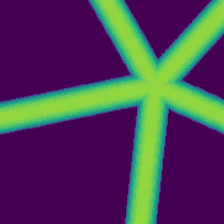
\includegraphics[width=36.0000bp,height=36.0000bp]{figures/pipeline_assets/asset_03.png}};
% Aligned label normal example
\node[anchor=north west,inner sep=0pt] at (969.8400,396.7200) {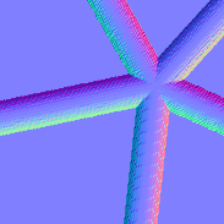
\includegraphics[width=36.0000bp,height=36.0000bp]{figures/pipeline_assets/asset_04.png}};
% Aligned planar-pose target schematic / background
\path[fill=pc10,draw=pc11,line width=0.8000bp,rounded corners=0.900bp] (1015.2000,396.7200) rectangle (1051.2000,432.7200);
% Aligned planar-pose target schematic / x axis
\draw[draw=pc12,line width=1.0000bp,line cap=round,-{Triangle[length=3.4bp,width=3bp]}] (1023.8399,424.4400) -- (1045.0799,424.4400);
% Aligned planar-pose target schematic / y axis
\draw[draw=pc12,line width=1.0000bp,line cap=round,-{Triangle[length=3.4bp,width=3bp]}] (1023.8399,424.4400) -- (1023.8399,402.4800);
% Aligned planar-pose target schematic / pose frame 0
\draw[draw=pc13,line width=1.0000bp,line cap=round] (1026.3374,414.4587) -- (1040.5321,405.9297);
% Aligned planar-pose target schematic / pose frame 1
\draw[draw=pc13,line width=1.0000bp,line cap=round] (1040.5321,405.9297) -- (1042.9425,409.9412);
% Aligned planar-pose target schematic / pose frame 2
\draw[draw=pc13,line width=1.0000bp,line cap=round] (1042.9425,409.9412) -- (1028.7478,418.4702);
% Aligned planar-pose target schematic / pose frame 3
\draw[draw=pc13,line width=1.0000bp,line cap=round] (1028.7478,418.4702) -- (1026.3374,414.4587);
% Aligned planar-pose target schematic / origin
\path[fill=pc13,draw=pc13,line width=1.0000bp] (1023.8399,424.4399) ellipse [x radius=0.9720bp,y radius=0.9720bp];
% Aligned targets caption
\node[anchor=center,inner sep=0pt,text=pc13,font=\fontsize{20.00bp}{22.40bp}\selectfont] at (987.8400,451.4400) {Pseudo-labels};
% Geometry targets supervise student
\draw[draw=pc1,line width=1.0000bp,line cap=round,dash pattern=on 3bp off 2.5bp,-{Triangle[length=3.4bp,width=3bp]}] (599.0400,419.0400) -- (359.2800,419.0400);
% Supervision arrow caption
\node[anchor=center,inner sep=0pt,text=pc13,font=\fontsize{20.00bp}{22.40bp}\selectfont] at (479.5200,402.8399) {Geometric supervision};
% Panel divider
\draw[draw=pc6,line width=0.7500bp,line cap=round] (25.2000,483.8400) -- (1125.3600,483.8400);
% Panel b heading
\node[anchor=west,inner sep=0pt,text=pc2,font=\fontsize{26.00bp}{29.12bp}\selectfont] at (25.2000,508.3200) {\textbf{(b) Inference}};
% Inference real tactile image
\node[anchor=north west,inner sep=0pt] at (41.7600,547.9200) {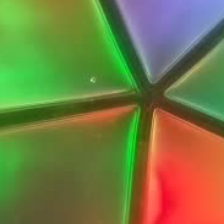
\includegraphics[width=52.5600bp,height=52.5600bp]{figures/pipeline_assets/asset_01.png}};
% Inference inputs
\node[anchor=center,inner sep=0pt,text=pc7,font=\fontsize{21.00bp}{23.52bp}\selectfont] at (122.4000,574.5600) {$\Tactile,\,o$};
% Inference input to student
\draw[draw=pc8,line width=0.8500bp,line cap=round,-{Triangle[length=3.4bp,width=3bp]}] (142.5600,574.5600) -- (174.9600,574.5600);
% Student inference module
\path[fill=pc5,draw=pc6,line width=0.8500bp,rounded corners=1.728bp] (175.6800,545.0400) rectangle (324.0000,602.6400);
% Student to predicted geometry
\draw[draw=pc8,line width=0.8500bp,line cap=round,-{Triangle[length=3.4bp,width=3bp]}] (324.7200,574.5600) -- (362.8800,574.5600);
% Predicted depth illustration
\node[anchor=north west,inner sep=0pt] at (368.6400,546.4800) {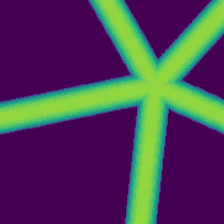
\includegraphics[width=48.9600bp,height=48.9600bp]{figures/pipeline_assets/asset_03.png}};
% Predicted normals illustration
\node[anchor=north west,inner sep=0pt] at (443.5200,546.4800) {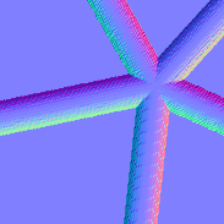
\includegraphics[width=48.9600bp,height=48.9600bp]{figures/pipeline_assets/asset_04.png}};
% Predicted planar pose schematic / x axis
\draw[draw=pc12,line width=0.7500bp,line cap=round,-{Triangle[length=3.4bp,width=3bp]}] (529.4304,584.1791) -- (558.3168,584.1791);
% Predicted planar pose schematic / y axis
\draw[draw=pc12,line width=0.7500bp,line cap=round,-{Triangle[length=3.4bp,width=3bp]}] (529.4304,584.1791) -- (529.4304,554.3135);
% Predicted planar pose schematic / pose frame 0
\draw[draw=pc13,line width=1.1000bp,line cap=round] (532.8269,570.6046) -- (552.1317,559.0052);
% Predicted planar pose schematic / pose frame 1
\draw[draw=pc13,line width=1.1000bp,line cap=round] (552.1317,559.0052) -- (555.4098,564.4609);
% Predicted planar pose schematic / pose frame 2
\draw[draw=pc13,line width=1.1000bp,line cap=round] (555.4098,564.4609) -- (536.1050,576.0603);
% Predicted planar pose schematic / pose frame 3
\draw[draw=pc13,line width=1.1000bp,line cap=round] (536.1050,576.0603) -- (532.8269,570.6046);
% Predicted planar pose schematic / origin
\path[fill=pc13,draw=pc13,line width=1.0000bp] (529.4303,584.1791) ellipse [x radius=1.3219bp,y radius=1.3219bp];
% Inference depth caption
\node[anchor=center,inner sep=0pt,text=pc2,font=\fontsize{20.00bp}{22.40bp}\selectfont] at (393.1200,608.0400) {Depth};
% Inference normals caption
\node[anchor=center,inner sep=0pt,text=pc2,font=\fontsize{20.00bp}{22.40bp}\selectfont] at (468.7200,608.0400) {Normals};
% Inference pose caption
\node[anchor=center,inner sep=0pt,text=pc2,font=\fontsize{20.00bp}{22.40bp}\selectfont] at (542.1600,608.0400) {Pose};
% Optional pose refinement boundary
\path[fill=pc14,draw=pc15,line width=0.7500bp,dash pattern=on 3bp off 2.5bp,rounded corners=2.163bp] (628.5600,501.1200) rectangle (1125.3600,621.3600);
% Optional branch heading
\node[anchor=center,inner sep=0pt,text=pc12,font=\fontsize{20.00bp}{22.40bp}\selectfont] at (876.2400,516.9600) {Pose refinement (optional)};
% Optional branch initial state
\node[anchor=center,inner sep=0pt,text=pc7,font=\fontsize{20.00bp}{22.40bp}\selectfont] at (665.2800,556.5600) {$q_0$};
% Optional refinement real image
\node[anchor=north west,inner sep=0pt] at (797.7600,534.2400) {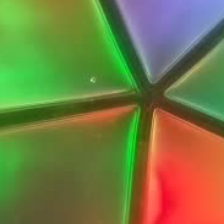
\includegraphics[width=18.0000bp,height=18.0000bp]{figures/pipeline_assets/asset_01.png}};
% Optional refinement object mesh
\node[anchor=north west,inner sep=0pt] at (825.1200,534.2400) {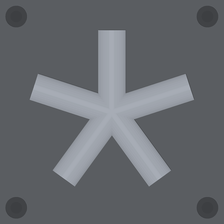
\includegraphics[width=18.0000bp,height=18.0000bp]{figures/pipeline_assets/asset_02.png}};
% Reused residual aligner module
\path[fill=pc5,draw=pc9,line width=0.8500bp,rounded corners=1.498bp] (764.6400,555.8400) rectangle (891.3600,593.2800);
% Optional aligner name
\node[anchor=center,inner sep=0pt,text=pc4,font=\fontsize{22.00bp}{24.64bp}\selectfont] at (828.0000,573.8400) {\textbf{Aligner}~$\Aligner$};
% Refined planar pose schematic / x axis
\draw[draw=pc12,line width=1.0000bp,line cap=round,-{Triangle[length=3.4bp,width=3bp]}] (960.7104,584.1791) -- (989.5968,584.1791);
% Refined planar pose schematic / y axis
\draw[draw=pc12,line width=1.0000bp,line cap=round,-{Triangle[length=3.4bp,width=3bp]}] (960.7104,584.1791) -- (960.7104,554.3135);
% Refined planar pose schematic / pose frame 0
\draw[draw=pc13,line width=1.0000bp,line cap=round] (964.1069,570.6046) -- (983.4117,559.0052);
% Refined planar pose schematic / pose frame 1
\draw[draw=pc13,line width=1.0000bp,line cap=round] (983.4117,559.0052) -- (986.6898,564.4609);
% Refined planar pose schematic / pose frame 2
\draw[draw=pc13,line width=1.0000bp,line cap=round] (986.6898,564.4609) -- (967.3850,576.0603);
% Refined planar pose schematic / pose frame 3
\draw[draw=pc13,line width=1.0000bp,line cap=round] (967.3850,576.0603) -- (964.1069,570.6046);
% Refined planar pose schematic / origin
\path[fill=pc13,draw=pc13,line width=1.0000bp] (960.7103,584.1791) ellipse [x radius=1.3219bp,y radius=1.3219bp];
% Refined output caption
\node[anchor=center,inner sep=0pt,text=pc2,font=\fontsize{20.00bp}{22.40bp}\selectfont] at (1064.1600,574.5600) {Refined pose};
% Registered contacts heading
\node[anchor=west,inner sep=0pt,text=pc2,font=\fontsize{23.00bp}{25.76bp}\selectfont] at (25.2000,84.2400) {\textbf{Labeled contacts}};
% Registered tactile observation I
\node[anchor=north west,inner sep=0pt] at (40.3200,108.7200) {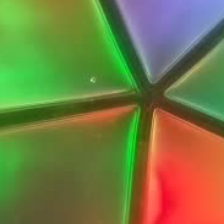
\includegraphics[width=40.3200bp,height=40.3200bp]{figures/pipeline_assets/asset_01.png}};
% Registered object mesh M
\node[anchor=north west,inner sep=0pt] at (102.9600,108.7200) {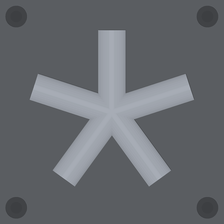
\includegraphics[width=40.3200bp,height=40.3200bp]{figures/pipeline_assets/asset_02.png}};
% Registered input I
\node[anchor=center,inner sep=0pt,text=pc7,font=\fontsize{20.00bp}{22.40bp}\selectfont] at (60.4800,163.8000) {$\Tactile$};
% Registered input M
\node[anchor=center,inner sep=0pt,text=pc7,font=\fontsize{20.00bp}{22.40bp}\selectfont] at (123.1200,163.8000) {$\Mesh$};
% Registered state x axis
\draw[draw=pc7,line width=0.6500bp,line cap=round,-{Triangle[length=3.4bp,width=3bp]}] (171.3600,145.4400) -- (230.4000,145.4400);
% Registered state y axis
\draw[draw=pc7,line width=0.6500bp,line cap=round,-{Triangle[length=3.4bp,width=3bp]}] (171.3600,145.4400) -- (171.3600,105.8400);
% Registered state schematic edge 1
\draw[draw=pc7,line width=1.1000bp,line cap=round] (181.1593,131.6587) -- (218.9428,110.7149);
% Registered state schematic edge 2
\draw[draw=pc7,line width=1.1000bp,line cap=round] (218.9428,110.7149) -- (223.4806,118.9013);
% Registered state schematic edge 3
\draw[draw=pc7,line width=1.1000bp,line cap=round] (223.4806,118.9013) -- (185.6971,139.8450);
% Registered state schematic edge 4
\draw[draw=pc7,line width=1.1000bp,line cap=round] (185.6971,139.8450) -- (181.1593,131.6587);
% Registered state q star
\node[anchor=center,inner sep=0pt,text=pc7,font=\fontsize{20.00bp}{22.40bp}\selectfont] at (200.1600,163.8000) {$q^\ast$};
% Registered state and mesh to perturbation
\draw[draw=pc7,line width=0.9500bp,line cap=round,-{Triangle[length=3.4bp,width=3bp]}] (247.6800,134.6400) -- (328.3199,134.6400);
% Registered supervision trains teacher
\draw[draw=pc7,line width=0.9500bp,line cap=round,dash pattern=on 3bp off 2.5bp,-{Triangle[length=3.4bp,width=3bp]}] (209.5200,181.4400) -- (209.5200,257.0400);
% Teacher training connection
\node[anchor=west,inner sep=0pt,text=pc7,font=\fontsize{18.00bp}{20.16bp}\selectfont] at (217.4400,217.4400) {train};
% Perturb and project stage
\node[anchor=center,inner sep=0pt,text=pc4,font=\fontsize{19.00bp}{21.28bp}\selectfont] at (395.2799,108.3600) {\textbf{Perturb + project}};
% Original registered state ghost edge 1
\draw[draw=pc16,line width=1.0000bp,line cap=round,dash pattern=on 3bp off 2.5bp] (347.0066,145.2656) -- (401.0430,124.5788);
% Original registered state ghost edge 2
\draw[draw=pc16,line width=1.0000bp,line cap=round,dash pattern=on 3bp off 2.5bp] (401.0430,124.5788) -- (406.1133,131.4446);
% Original registered state ghost edge 3
\draw[draw=pc16,line width=1.0000bp,line cap=round,dash pattern=on 3bp off 2.5bp] (406.1133,131.4446) -- (352.0769,152.1314);
% Original registered state ghost edge 4
\draw[draw=pc16,line width=1.0000bp,line cap=round,dash pattern=on 3bp off 2.5bp] (352.0769,152.1313) -- (347.0066,145.2656);
% Perturbed candidate state edge 1
\draw[draw=pc4,line width=1.4500bp,line cap=round] (363.5062,130.8320) -- (424.1106,124.6994);
% Perturbed candidate state edge 2
\draw[draw=pc4,line width=1.4500bp,line cap=round] (424.1106,124.6994) -- (425.6137,132.3998);
% Perturbed candidate state edge 3
\draw[draw=pc4,line width=1.4500bp,line cap=round] (425.6137,132.3998) -- (365.0093,138.5324);
% Perturbed candidate state edge 4
\draw[draw=pc4,line width=1.4500bp,line cap=round] (365.0093,138.5324) -- (363.5062,130.8320);
% Geometric displacement delta
\draw[draw=pc4,line width=1.0000bp,line cap=round,-{Triangle[length=3.4bp,width=3bp]}] (364.3200,146.6495) -- (391.6800,140.9471);
% State perturbation delta
\node[anchor=west,inner sep=0pt,text=pc4,font=\fontsize{19.00bp}{21.28bp}\selectfont] at (403.2000,148.7231) {$\delta$};
% Projected perturbed depth
\node[anchor=center,inner sep=0pt,text=pc7,font=\fontsize{19.00bp}{21.28bp}\selectfont] at (395.2800,173.8800) {$d(\Mesh,q^\ast+\delta)$};
% Aligner training module
\path[fill=pc5,draw=pc4,line width=1.2000bp,rounded corners=1.764bp] (505.4400,149.0399) rectangle (636.4800,199.4399);
% Aligner training module label
\node[anchor=center,inner sep=0pt,text=pc4,font=\fontsize{22.00bp}{24.64bp}\selectfont] at (570.9600,173.8799) {\textbf{Aligner}~$\Aligner$};
% Real tactile observation for aligner training
\node[anchor=north west,inner sep=0pt] at (551.5200,102.9600) {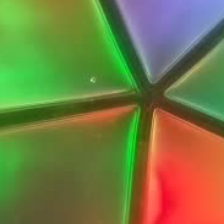
\includegraphics[width=28.0800bp,height=28.0800bp]{figures/pipeline_assets/asset_01.png}};
% Real tactile training input symbol
\node[anchor=west,inner sep=0pt,text=pc7,font=\fontsize{20.00bp}{22.40bp}\selectfont] at (586.0800,115.9200) {$\Tactile$};
% Known corrective target label
\node[anchor=center,inner sep=0pt,text=pc4,font=\fontsize{18.00bp}{20.16bp}\selectfont] at (748.0800,116.6400) {Correction target};
% Correction learning target
\path[fill=pc5,draw=pc17,line width=0.9000bp,rounded corners=1.764bp] (692.6400,149.0399) rectangle (806.4000,199.4399);
% Corrective supervision delta
\node[anchor=center,inner sep=0pt,text=pc4,font=\fontsize{22.00bp}{24.64bp}\selectfont] at (749.5200,173.8799) {$\Delta q\approx-\delta$};
% Weight reuse label
\node[anchor=west,inner sep=0pt,text=pc4,font=\fontsize{17.50bp}{19.60bp}\selectfont] at (534.2400,219.2400) {\textit{reuse}~$\Aligner$};
% Perturbed state projected to depth
\draw[draw=pc4,line width=0.9000bp,line cap=round,-{Triangle[length=3.4bp,width=3bp]}] (393.1200,151.2000) -- (393.1200,159.1200);
% Perturbed depth enters training aligner
\draw[draw=pc4,line width=1.0000bp,line cap=round,-{Triangle[length=3.4bp,width=3bp]}] (465.8400,174.2400) -- (504.0000,174.2400);
% Aligner predicts residual for known corrective target
\draw[draw=pc4,line width=1.0000bp,line cap=round,-{Triangle[length=3.4bp,width=3bp]}] (637.9199,174.2400) -- (691.2000,174.2400);
% Real image enters training aligner
\draw[draw=pc12,line width=0.9000bp,line cap=round,-{Triangle[length=3.4bp,width=3bp]}] (565.5600,133.2000) -- (565.5600,147.5999);
% Reuse learned aligner weights
\draw[draw=pc4,line width=0.9500bp,line cap=round,dash pattern=on 3bp off 2.5bp,-{Triangle[length=3.4bp,width=3bp]}] (525.6000,200.8800) -- (525.6000,257.0400);
% Image and mesh to optional aligner
\draw[draw=pc12,line width=0.9000bp,line cap=round,-{Triangle[length=3.4bp,width=3bp]}] (820.8000,552.6000) -- (820.8000,555.1200);
% Horizontal initialization arrow
\draw[draw=pc12,line width=1.1000bp,line cap=round,-{Triangle[length=3.4bp,width=3bp]}] (580.3200,574.5600) -- (763.2000,574.5600);
% Optional aligner to refined pose
\draw[draw=pc12,line width=1.0000bp,line cap=round,-{Triangle[length=3.4bp,width=3bp]}] (892.8000,574.5600) -- (943.2000,574.5600);
% Teacher / role label (Teacher module)
% Teacher / mathematical model (Teacher module)
\node[anchor=center,inner sep=0pt,text=pc18,font=\fontsize{20.00bp}{22.40bp}\selectfont] at (209.5200,286.9200) {\textbf{Teacher}~$\Teacher$};
% Student / role label (Student training module)
% Student / mathematical model (Student training module)
\node[anchor=center,inner sep=0pt,text=pc18,font=\fontsize{20.00bp}{22.40bp}\selectfont] at (276.8400,419.7600) {\textbf{Student}~$\Student$};
% Student / role label (Student inference module)
% Student / mathematical model (Student inference module)
\node[anchor=center,inner sep=0pt,text=pc18,font=\fontsize{20.00bp}{22.40bp}\selectfont] at (249.8400,573.8400) {\textbf{Student}~$\Student$};
% Aligned pseudo-labels / heading
\node[anchor=center,inner sep=0pt,text=pc13,font=\fontsize{23.00bp}{25.76bp}\selectfont] at (1000.0800,82.0800) {\textbf{Aligned pseudo-labels}};
% Known mesh for geometric targets
\node[anchor=north west,inner sep=0pt] at (936.0000,111.6000) {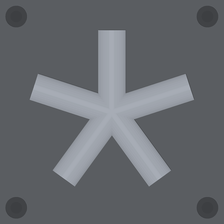
\includegraphics[width=34.5600bp,height=34.5600bp]{figures/pipeline_assets/asset_02.png}};
% Known mesh for targets / label
\node[anchor=west,inner sep=0pt,text=pc7,font=\fontsize{20.00bp}{22.40bp}\selectfont] at (978.4800,126.3600) {Mesh~$\Mesh$};
% Known mesh enters target generator
\draw[draw=pc13,line width=0.9000bp,line cap=round,-{Triangle[length=3.4bp,width=3bp]}] (1000.0800,149.7600) -- (1000.0800,162.7199);
% Geometric target generator
\path[fill=pc5,draw=pc19,line width=0.8000bp,rounded corners=1.814bp] (903.6000,165.6000) rectangle (1098.0000,226.0800);
% Geometric target generator / name
\node[anchor=center,inner sep=0pt,text=pc2,font=\fontsize{21.00bp}{23.52bp}\selectfont] at (1000.8000,182.8800) {\textbf{Geometric targets}};
% Geometric target generator / map
\node[anchor=center,inner sep=0pt,text=pc13,font=\fontsize{20.00bp}{22.40bp}\selectfont] at (1000.8000,209.8800) {$\Targets(\Mesh,q_T)$};
% Aligned state into target generator / outlet
\draw[draw=pc7,line width=0.9000bp,line cap=round] (806.4000,287.2800) -- (850.3200,287.2800);
% Aligned state into target generator / rise
\draw[draw=pc7,line width=0.9000bp,line cap=round] (850.3200,287.2800) -- (850.3200,195.8400);
% Aligned state into target generator / input
\draw[draw=pc7,line width=0.9000bp,line cap=round,-{Triangle[length=3.4bp,width=3bp]}] (850.3200,195.8400) -- (902.1600,195.8400);
% Aligned state q_T
\node[anchor=center,inner sep=0pt,text=pc7,font=\fontsize{21.00bp}{23.52bp}\selectfont] at (837.7200,268.5600) {$q_T$};
% Geometric target generator to outputs
\draw[draw=pc13,line width=0.9000bp,line cap=round,-{Triangle[length=3.4bp,width=3bp]}] (1000.0800,227.5200) -- (1000.0800,249.1200);
% Depth pseudo-label: original projected geometry
\node[anchor=north west,inner sep=0pt] at (891.3600,258.4800) {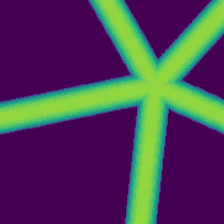
\includegraphics[width=58.3200bp,height=58.3200bp]{figures/pipeline_assets/asset_03.png}};
% Normal pseudo-label: original projected geometry
\node[anchor=north west,inner sep=0pt] at (969.8400,258.4800) {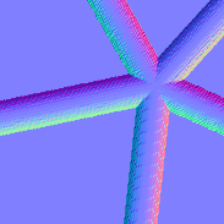
\includegraphics[width=58.3200bp,height=58.3200bp]{figures/pipeline_assets/asset_04.png}};
% Planar-pose pseudo-label schematic / background
\path[fill=pc10,draw=pc11,line width=0.8000bp,rounded corners=1.458bp] (1049.0400,258.4800) rectangle (1107.3600,316.8000);
% Planar-pose pseudo-label schematic / x axis
\draw[draw=pc12,line width=1.0000bp,line cap=round,-{Triangle[length=3.4bp,width=3bp]}] (1063.0368,303.3863) -- (1097.4455,303.3863);
% Planar-pose pseudo-label schematic / y axis
\draw[draw=pc12,line width=1.0000bp,line cap=round,-{Triangle[length=3.4bp,width=3bp]}] (1063.0368,303.3863) -- (1063.0368,267.8111);
% Planar-pose pseudo-label schematic / pose frame 0
\draw[draw=pc13,line width=1.0000bp,line cap=round] (1067.0826,287.2167) -- (1090.0780,273.3997);
% Planar-pose pseudo-label schematic / pose frame 1
\draw[draw=pc13,line width=1.0000bp,line cap=round] (1090.0780,273.3997) -- (1093.9828,279.8983);
% Planar-pose pseudo-label schematic / pose frame 2
\draw[draw=pc13,line width=1.0000bp,line cap=round] (1093.9828,279.8983) -- (1070.9874,293.7154);
% Planar-pose pseudo-label schematic / pose frame 3
\draw[draw=pc13,line width=1.0000bp,line cap=round] (1070.9874,293.7154) -- (1067.0826,287.2167);
% Planar-pose pseudo-label schematic / origin
\path[fill=pc13,draw=pc13,line width=1.0000bp] (1063.0368,303.3864) ellipse [x radius=1.5746bp,y radius=1.5746bp];
% Geometric output / Depth
\node[anchor=center,inner sep=0pt,text=pc2,font=\fontsize{21.00bp}{23.52bp}\selectfont] at (921.6000,335.1600) {Depth};
% Geometric output / Normals
\node[anchor=center,inner sep=0pt,text=pc2,font=\fontsize{21.00bp}{23.52bp}\selectfont] at (1000.0800,335.1600) {Normals};
% Geometric output / Pose
\node[anchor=center,inner sep=0pt,text=pc2,font=\fontsize{21.00bp}{23.52bp}\selectfont] at (1080.0000,335.1600) {Pose};
% Pseudo-labels enter student supervision
\draw[draw=pc13,line width=0.9000bp,line cap=round,dash pattern=on 3bp off 2.5bp,-{Triangle[length=3.4bp,width=3bp]}] (1000.0800,364.3200) -- (1000.0800,385.2000);
\end{scope}
\end{tikzpicture}%
